\subsection{Muestreo}

Para esta sección se considera la señal de tiempo continuo $s(t) = sin(2\pi t)$, muestreada a intervalos uniformes $T_s$.

\begin{enumerate}
    
    %1
    \item Usando $T_s = 1/10$ y $ 0 \leq n \leq 100 $ se tiene:
    $$s_1[n] = \sin\left(2\pi \dfrac{1}{10}n\right)$$
    cuyo gráfico utilizando el comando \texttt{stem} se muestra en la figura \ref{fig:Ip2}.
    
    %2
    \item Usando $T_s = 1/3$ y $ 0 \leq n \leq 30 $ se tiene:
    $$s_2[n] = \sin\left(2\pi \dfrac{1}{3}n\right)$$
    cuyo gráfico utilizando el comando \texttt{stem} se muestra en la figura \ref{fig:Ip2}.
    
    %3
    \item Usando $T_s = 1/2$ y $ 0 \leq n \leq 20 $ se tiene:
    $$s_3[n] = \sin\left(2\pi \dfrac{1}{2}n\right)$$
    cuyo gráfico utilizando el comando \texttt{stem} se muestra en la figura \ref{fig:Ip2}.
    
    %4
    \item Usando $T_s = 10/9$ y $ 0 \leq n \leq 9 $ se tiene:
    $$s_4[n] = \sin\left(2\pi \dfrac{10}{9}n\right)$$
    cuyo gráfico utilizando el comando \texttt{stem} se muestra en la figura \ref{fig:Ip2}.
    
    \begin{figure}[H]
    \centering
    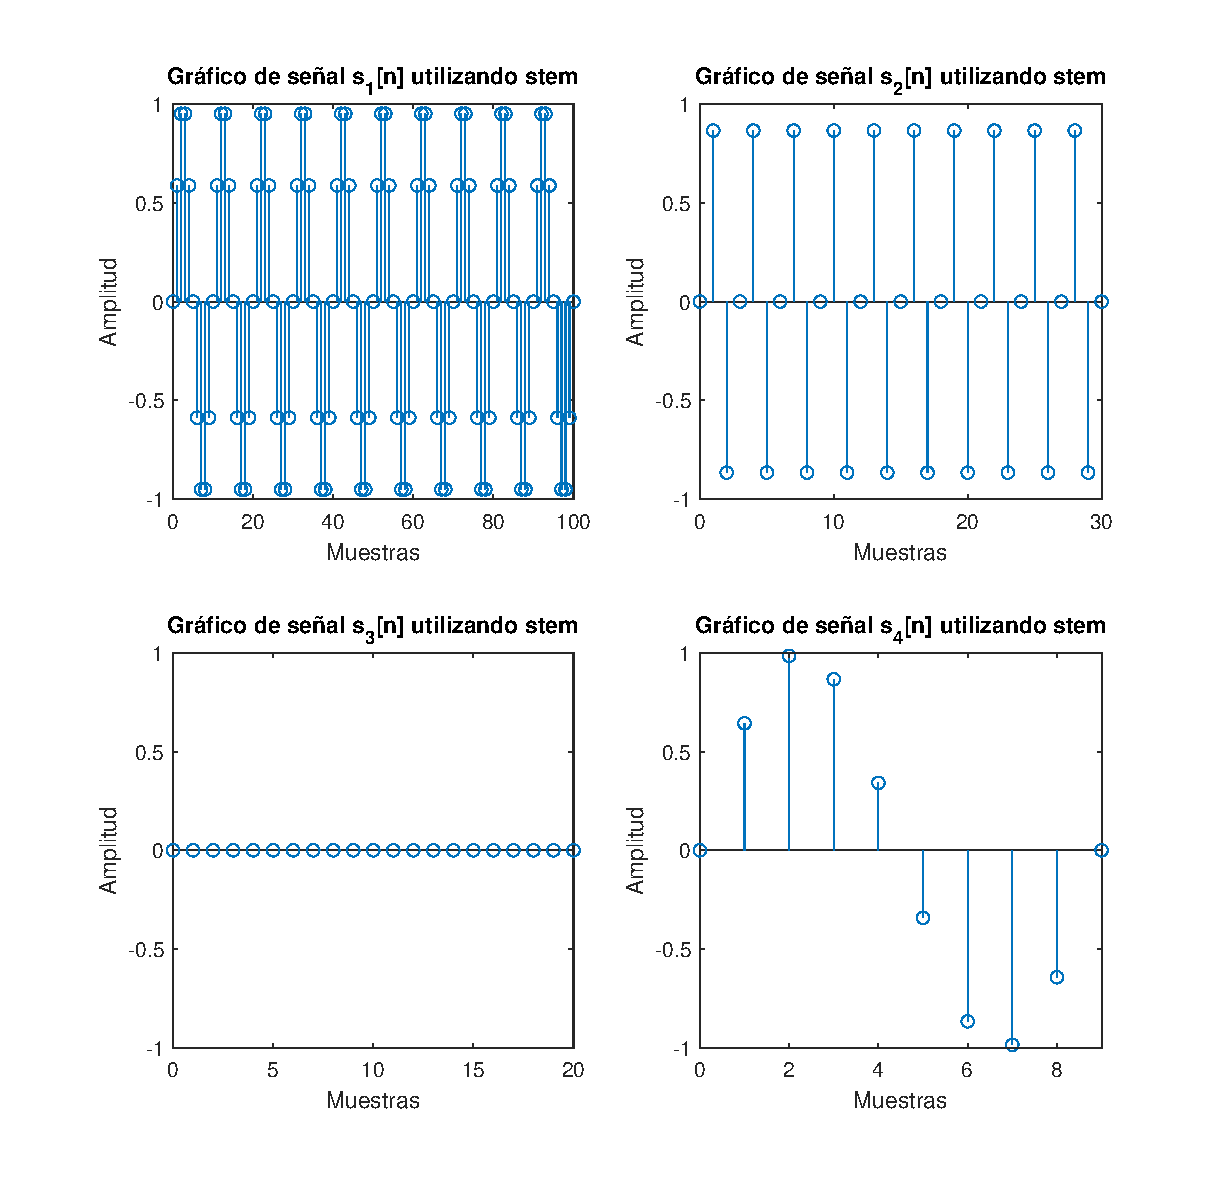
\includegraphics[scale = 0.7]{Imagenes/muestreo_sennales.eps}
    \caption{Señales de tiempo discreto $s_1[n]$, $s_2[n]$, $s_3[n]$ y $s_4[n]$.}
    \label{fig:Ip2}
    \end{figure}
    
    %5
    \item La frecuencia de cada señal de tiempo discreto en ciclos por muestra corresponde a:
    $$ f_r = f \cdot T_s = T_s$$
    donde $f$ corresponde a la frecuencia de la señal de tiempo continuo.
    Por lo anterior la frecuencia de las señales de tiempo discreto obtenidas son:
    
    \begin{itemize}
        \item $s_1[n]$: $1/10$ ciclos por muestra.
        \item $s_2[n]$: $1/3$ ciclos por muestra.
        \item $s_3[n]$: $1/2$ ciclos por muestra. 
        \item $s_4[n]$: $10/9$ ciclos por muestra.
    \end{itemize}
    
    %6
    \item Las muestras por periodo, considerando un periodo de 1 s en la señal de tiempo continuo, corresponde a:
    $$ \text{muestras por periodo}  = \dfrac{T}{T_s} = \dfrac{1 s}{ T_s} $$
    donde $f$ corresponde a la frecuencia (Hz) en tiempo continuo. De lo anterior se concluye que:
    
    \begin{itemize}
        \item $s_1[n]$: 10 muestras por periodo
        \item $s_2[n]$: 3 muestras por periodo
        \item $s_3[n]$: 2 muestras por periodo
        \item $s_4[n]$: 0.9 muestras por periodo.
    \end{itemize}
    
    %7
    \item En términos de series de tiempo, claramente las señales no son equivalentes, pues son secuencias distintas pues tienen valores numéricos distintos para los mismos valores del eje x.
    
    En términos de reconstrucción de la señal de tiempo continuo, las señales $s_1[n]$ y $s_2[n]$ son equivalentes, pues cumplen el criterio de nyquist.
    
    %8
    \item La frecuencia de muestreo $f_s$ (sps) que generan cada una de las señales corresponde a:
    $$ f_s = 1/T_s$$
    de lo anterior se concluye que:
    
    \begin{itemize}
        \item $s_1[n]$: 10 sps
        \item $s_2[n]$: 3 sps
        \item $s_3[n]$: 2 sps
        \item $s_4[n]$: 0.9 sps
    \end{itemize}
    
    lo que numéricamente coincide con las muestras por periodo. Esto es debido a que el periodo de la señal de tiempo continuo es de 1 segundo.
    
    %9
    \item La resolución de muestreo afecta a la frecuencia de la señal de tiempo discreto ($f_r$) de la siguiente forma:
    $$ f_r = f/f_s$$
    donde $f$ corresponde a la frecuencia de la señal en tiempo continuo y $f_s$ a la frecuencia de muestreo.
    
    Mas importante que la expresión anterior es el doblaje de frecuencias, donde al no cumplir estrictamente el criterio de nyquist, es decir:
    
    $$ f_r \leq 0.5$$
    
    no se es capaz de distinguir la frecuencia de la señal de tiempo continuo con respecto a otra en el intervalo $[0 ; f_s/2]$.
    
    Dicho efecto ocurre en la señal $s_4[n]$. Aquí $f_s$ es mayor a las demás señales (observar parte 5.) sin embargo, en la figura \ref{fig:Ip2} se observa una frecuencia menor. 
    
    Para obtener la frecuencia observada en $s_4[n]$ ($f_{\text{obs}}$) se calcula:
    
    $$ f_{\text{obs}} = (f_r - 1) = \dfrac{10}{9}-1 = 1/9 $$
    
    expresión que se concluyó a partir del diagrama de doblaje de frecuencias, mostrado en la figura \ref{fig:Ip2df}.
    
    \begin{figure}[H]
        \centering
        \includegraphics[width = .6 \linewidth]{Imagenes/Ip2_df.png}
        \caption{Diagrama de doblaje en frecuencias.}
        \label{fig:Ip2df}
    \end{figure}
    
    Cabe mencionar que el efecto en $s_3[n]$ de observar una frecuencia de 0 ciclos por muestra no corresponde a doblaje en frecuencia, sino que es debido a la fase de la sinusoide y a no cumplir el criterio de Nyquist.
    
    
    

    
\end{enumerate}



